\documentclass[tikz,border=10pt]{standalone}
% Shared preamble for the CenterTask panel files (panel_a/b/c.tex).
% Edit colours and node styles here, once.
\usepackage{amsmath}
\usetikzlibrary{arrows.meta,positioning,calc}

% category colours as in ColorCategoryMap.m: 1=Short/Orange, 2=Mid/Green, 3=Long/Blue
\definecolor{catShort}{RGB}{243,178,132}
\definecolor{catMid}{RGB}{158,209,172}
\definecolor{catLong}{RGB}{157,188,234}

\tikzset{ctpanel/.style={
  font=\sffamily,
  band/.style={rounded corners=6pt, fill=black!7, draw=none, inner sep=8pt, minimum height=1.15cm},
  unit/.style={circle, fill=catMid!60, draw=none, minimum size=0.95cm, inner sep=0pt},
  flow/.style={-{Latex[length=2.2mm]}, line width=0.8pt},
  rowlab/.style={anchor=east, font=\sffamily\large},
  now/.style={fill=catShort!55, rounded corners=3pt, inner sep=3pt},
  stage/.style={rounded corners=6pt, fill=black!8, draw=none, inner sep=8pt, minimum height=1.2cm, align=center},
  target/.style={circle, minimum size=0.9cm, inner sep=0pt, draw=none, font=\sffamily\scriptsize, text=black!75},
  axis/.style={line width=0.6pt},
}}


\begin{document}
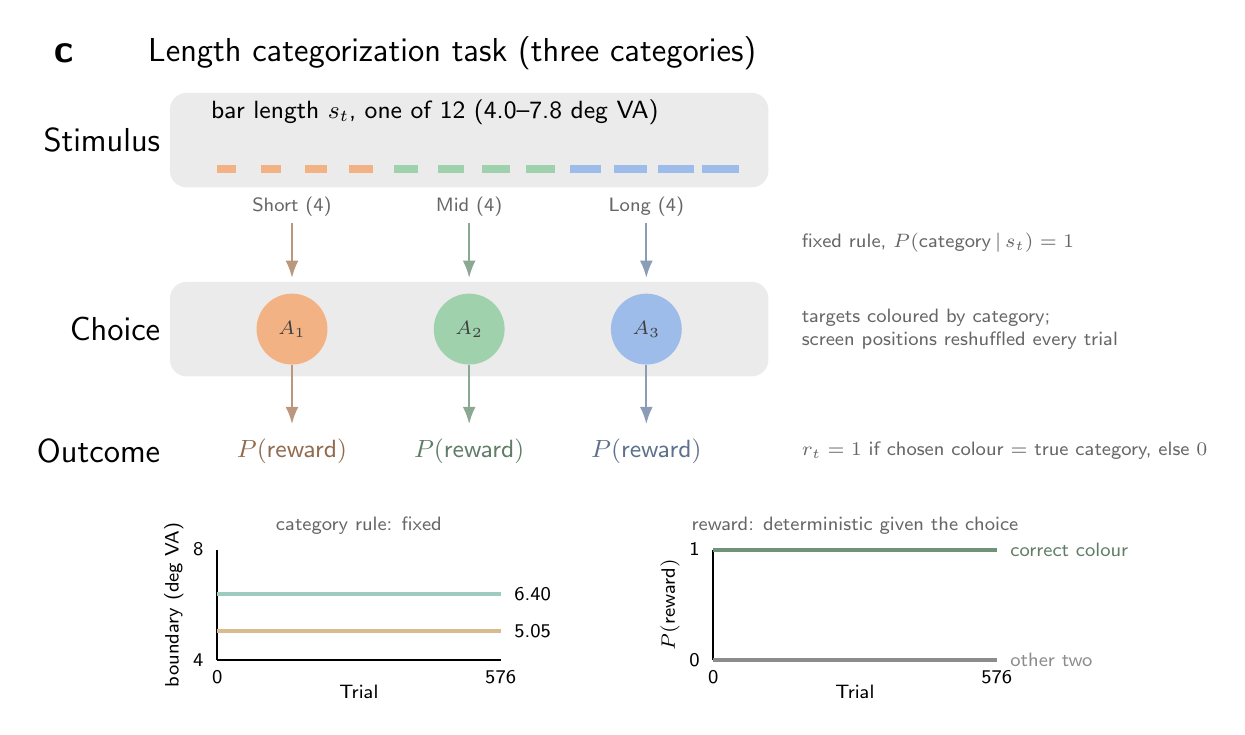
\begin{tikzpicture}[ctpanel]
% =====================================================================
%  (c)  Task structure of CenterTask, drawn like the reversal / two-stage tasks
% =====================================================================
\begin{scope}
\node[font=\sffamily\bfseries\Large, anchor=west] at (-2.2,1.1) {c};
\node[font=\sffamily\large, anchor=west] at (-1.0,1.1) {Length categorization task (three categories)};

% ---- stage labels ----
\node[rowlab] at (-0.6, 0)    {Stimulus};
\node[rowlab] at (-0.6,-2.4)  {Choice};
\node[rowlab] at (-0.6,-3.95) {Outcome};

% ---- Stage 1: bar length ----
\node[stage, minimum width=7.6cm] (stim) at (3.2,0) {};
\node[anchor=west, font=\sffamily\small] at (-0.2,0.35) {bar length $s_t$, one of 12 (4.0--7.8 deg VA)};
% twelve bars, 4 per category, growing in length
\foreach \i/\len/\col in {0/0.24/catShort,1/0.25/catShort,2/0.28/catShort,3/0.30/catShort,
                          4/0.31/catMid,5/0.34/catMid,6/0.36/catMid,7/0.37/catMid,
                          8/0.40/catLong,9/0.42/catLong,10/0.46/catLong,11/0.47/catLong}{
  \fill[\col] ({0.0+\i*0.56},{-0.42}) rectangle ++(\len,0.11);
}
\node[font=\sffamily\scriptsize, text=black!60] at (0.95,-0.85) {Short (4)};
\node[font=\sffamily\scriptsize, text=black!60] at (3.2,-0.85)  {Mid (4)};
\node[font=\sffamily\scriptsize, text=black!60] at (5.45,-0.85) {Long (4)};

% ---- arrows: every length maps deterministically to ONE category ----
\draw[flow, catShort!70!black!80] (0.95,-1.05) -- (0.95,-1.75);
\draw[flow, catMid!70!black!80]   (3.2,-1.05)  -- (3.2,-1.75);
\draw[flow, catLong!70!black!80]  (5.45,-1.05) -- (5.45,-1.75);
\node[font=\sffamily\scriptsize, text=black!60, anchor=west] at (7.3,-1.3) {fixed rule, $P(\text{category}\,|\,s_t)=1$};

% ---- Stage 2: three coloured targets ----
\node[stage, minimum width=7.6cm] (choice) at (3.2,-2.4) {};
\node[target, fill=catShort] (T1) at (0.95,-2.4) {$A_1$};
\node[target, fill=catMid]   (T2) at (3.2,-2.4)  {$A_2$};
\node[target, fill=catLong]  (T3) at (5.45,-2.4) {$A_3$};
\node[font=\sffamily\scriptsize, text=black!60, anchor=west, align=left] at (7.3,-2.4)
  {targets coloured by category;\\ screen positions reshuffled every trial};

% ---- Outcome ----
\draw[flow, catShort!70!black!80] (T1.south) -- ++(0,-0.75);
\draw[flow, catMid!70!black!80]   (T2.south) -- ++(0,-0.75);
\draw[flow, catLong!70!black!80]  (T3.south) -- ++(0,-0.75);
\node[font=\sffamily\small, text=catShort!60!black] at (0.95,-3.95) {$P(\text{reward})$};
\node[font=\sffamily\small, text=catMid!60!black]   at (3.2,-3.95)  {$P(\text{reward})$};
\node[font=\sffamily\small, text=catLong!60!black]  at (5.45,-3.95) {$P(\text{reward})$};
\node[font=\sffamily\scriptsize, text=black!60, anchor=west, align=left] at (7.3,-3.95)
  {$r_t = 1$ if chosen colour $=$ true category, else $0$};

% ---- small plots, as in panel d ----
% left: category boundary vs trial (flat: no reversal)
\begin{scope}[xshift=0.0cm, yshift=-6.6cm]
  \draw[axis] (0,0) -- (0,1.4);
  \draw[axis] (0,0) -- (3.6,0);
  \node[font=\sffamily\scriptsize, rotate=90] at (-0.55,0.7) {boundary (deg VA)};
  \node[font=\sffamily\scriptsize] at (1.8,-0.4) {Trial};
  \node[font=\sffamily\scriptsize, anchor=east] at (-0.05,0.0) {4};
  \node[font=\sffamily\scriptsize, anchor=east] at (-0.05,1.4) {8};
  \node[font=\sffamily\scriptsize] at (0,-0.22) {0};
  \node[font=\sffamily\scriptsize] at (3.6,-0.22) {576};
  % boundaries 5.05 and 6.40 mapped onto 4..8 -> 0..1.4
  \draw[line width=1.4pt, catShort!70!catMid] (0,0.3675) -- (3.6,0.3675);
  \draw[line width=1.4pt, catMid!70!catLong]  (0,0.84)   -- (3.6,0.84);
  \node[font=\sffamily\scriptsize, anchor=west] at (3.65,0.3675) {5.05};
  \node[font=\sffamily\scriptsize, anchor=west] at (3.65,0.84)   {6.40};
  \node[font=\sffamily\scriptsize, text=black!60] at (1.8,1.7) {category rule: fixed};
\end{scope}

% right: P(reward | choice) vs trial (deterministic 1 / 0)
\begin{scope}[xshift=6.3cm, yshift=-6.6cm]
  \draw[axis] (0,0) -- (0,1.4);
  \draw[axis] (0,0) -- (3.6,0);
  \node[font=\sffamily\scriptsize, rotate=90] at (-0.55,0.7) {$P(\text{reward})$};
  \node[font=\sffamily\scriptsize] at (1.8,-0.4) {Trial};
  \node[font=\sffamily\scriptsize, anchor=east] at (-0.05,0.0) {0};
  \node[font=\sffamily\scriptsize, anchor=east] at (-0.05,1.4) {1};
  \node[font=\sffamily\scriptsize] at (0,-0.22) {0};
  \node[font=\sffamily\scriptsize] at (3.6,-0.22) {576};
  \draw[line width=1.4pt, catMid!70!black] (0,1.4) -- (3.6,1.4);
  \draw[line width=1.4pt, black!45] (0,0.0) -- (3.6,0.0);
  \node[font=\sffamily\scriptsize, anchor=west, text=catMid!60!black] at (3.65,1.4) {correct colour};
  \node[font=\sffamily\scriptsize, anchor=west, text=black!45] at (3.65,0.0) {other two};
  \node[font=\sffamily\scriptsize, text=black!60] at (1.8,1.7) {reward: deterministic given the choice};
\end{scope}
\end{scope}
\end{tikzpicture}
\end{document}
